\section{GaitNet}

%%%%%%%%%%%%%%%%%%%%%%%%%%%%%%%%%%%%%%%%%%%%%%%%%%%%%%%%%%%%%%%%%%%%%%%%%%%%%%%%
\subsection{Architecture}

The footstep evaluation network is then used to feed the gait net
architecture shown in \autoref{fig:diagram-gaitnet-architecture}. The
gait net takes in the robot state information and ranked footstep
positions from the footstep evaluation network. It then outputs the
desired contact state\textemdash which feet should be in contact with
the ground. This information is then passed as constraints to the MPC.

\begin{figure}
  \centering
  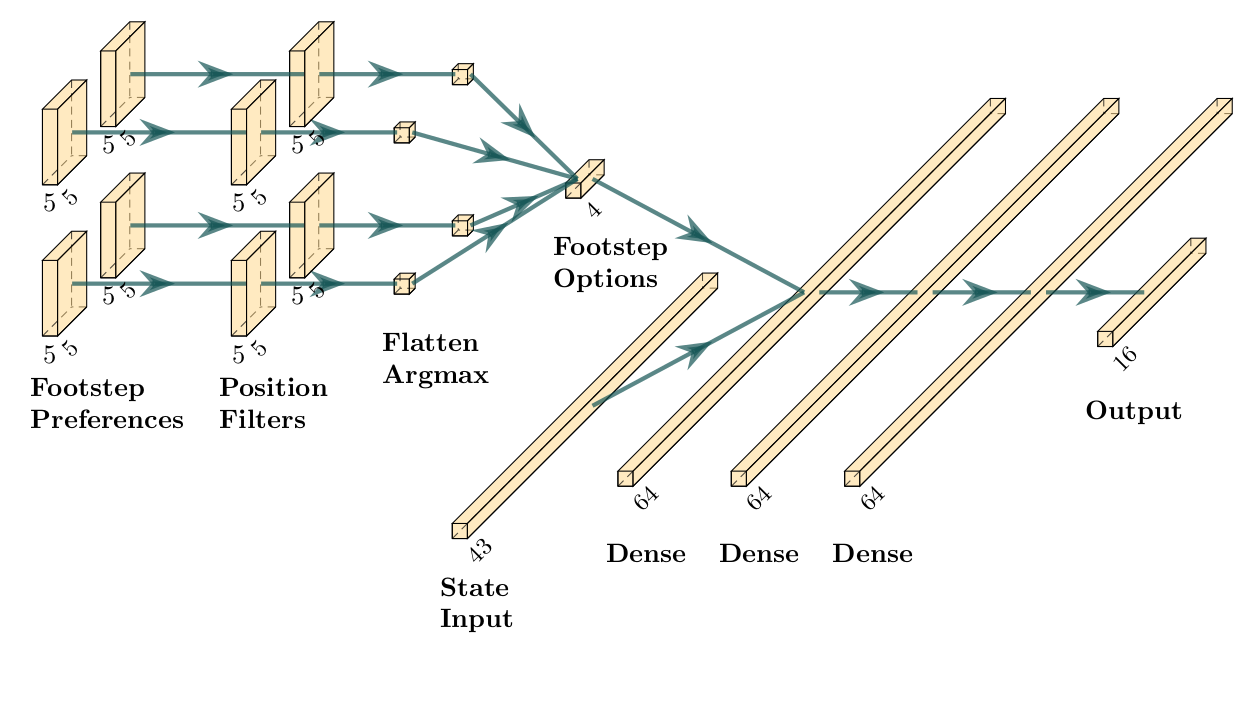
\includegraphics[width=0.75\linewidth]{images/diagrams/gait-network-architecture.png}
  \caption{Gait net architecture. Sections of the diagram include
    cost map pre-processing in yellow, footstep encoder in orange,
    state encoder in blue, and shared trunk in green. Cost maps for each
    foot are generated using ContactNet. The cost maps are then
    filtered based on the robot state and terrain data before being fed
    into the footstep encoder one at a time. The robot state is encoded
    before being combined with the footstep encodings in the shared
    trunk. The final output is the value of this option and the
  suggested swing duration.}
  \label{fig:diagram-gaitnet-architecture}
\end{figure}

The proposed model is designed to jointly evaluate robot state and
candidate footstep actions. The architecture consists of two
encoders, a shared trunk, and two task-specific output heads:
\begin{itemize}
  \item Robot state encoder. The robot state vector is processed by a
    two-layer feedforward encoder with intermediate dimensionality
    $d_{shared}$, each layer followed by Layer Normalization and ReLU
    activation.
    This produces a fixed-dimensional latent representation of the
    current state.
  \item Footstep encoder. Each candidate footstep, represented by the leg
    index (one-hot encoded), the relative displacement
    $(\delta x, \delta y)$, and an associated cost term, is encoded by a similar
    two-layer network with hidden size $d_{footstep}$, again using
    Layer Normalization and ReLU activations. Invalid or
    no-action candidates are handled through a learned embedding.
  \item Shared trunk. The concatenated robot state and footstep embeddings
    are processed by a two-layer feedforward “trunk,” reducing the
    dimensionality while applying Layer Normalization and ReLU nonlinearity.
  \item Output heads. From the shared trunk, two parallel prediction heads
    are applied

    \begin{itemize}
      \item a linear “value head” outputs the predicted reward
        value
      \item a one-layer “duration head” with sigmoid activation
        outputs a normalized swing duration, which is then scaled to the
        valid temporal range.
    \end{itemize}
\end{itemize}

This design allows the network to evaluate multiple candidate
footstep options in parallel, assigning each both an expected value
and a feasible swing duration, while explicitly supporting a
“no-action” option via a dedicated embedding.

\begin{todo}
  Use this somewhere:

  This network uses a multi-modal middle fusion
  architecture. This architecture was chosen to effectively combine the
  spatial features from the terrain data with the contextual features
  from the robot state data, while still maintaining flexibility in
  case re-training is needed \cite{feng2021deep}
\end{todo}

%%%%%%%%%%%%%%%%%%%%%%%%%%%%%%%%%%%%%%%%%%%%%%%%%%%%%%%%%%%%%%%%%%%%%%%%%%%%%%%%
\subsection{Training}
